\chapter{RESULTADOS E DISCUSSÕES}\label{cap:cap4}  
\section{RESULTADOS PARA O SISTEMA IEEE 33 BARRAS}
O sistema de 33 barras é um padrão de referência amplamente utilizado em estudos de fluxo de potência, planejamento e otimização de redes de distribuição elétrica. Consiste em 33 nós, interconectados por 32 linhas de distribuição, simulando uma rede de distribuição radial. Este sistema é caracterizado por um único ponto de alimentação (barra $V\theta$) e 32 barras de carga (barras $PQ$), representando a distribuição de energia elétrica de uma subestação para diversos consumidores finais. Os dados de barras e de linhas podem ser consultados no apêndice contendo todas as simulações e testes feitos.
\begin{figure}[H]
    \centering
    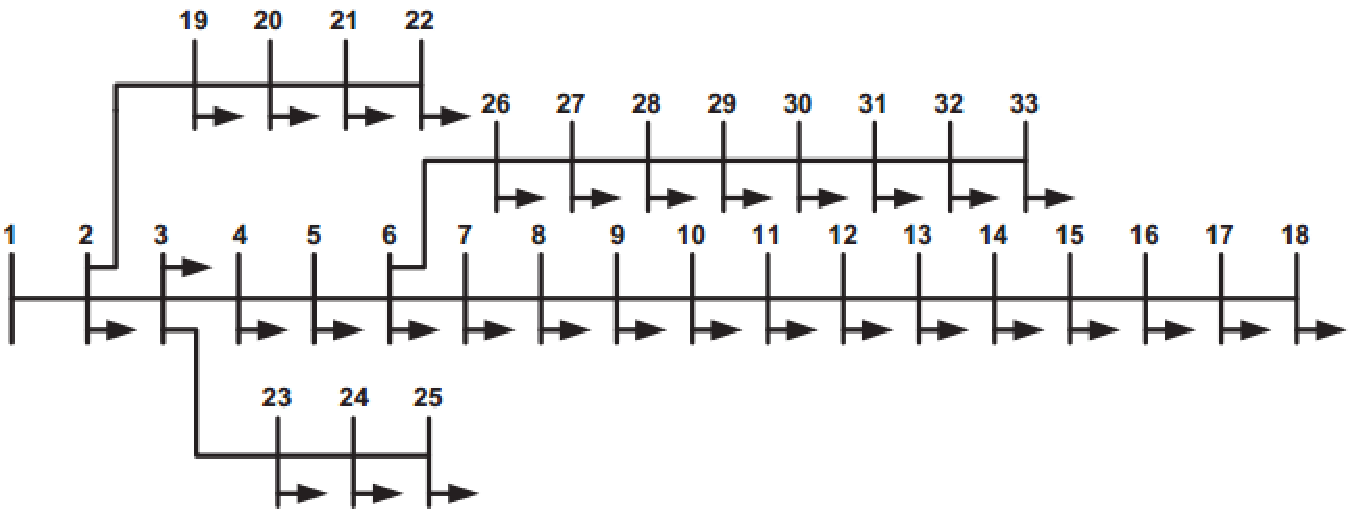
\includegraphics[scale=0.6]{textuais/capitulo4/figuras/IEEE_33BUS.pdf}
    \caption{Topologia do Sistema IEEE 33 Barras}
    \label{fig:14_BUS}
\end{figure}
\subsection{Análise Fractal}
Neste estudo, para obter os mapas fractais que possam ser analisados, foi necessário expandir a faixa de palpites iniciais muito além do usual para um \ac{FP}, indicando que todos os três métodos têm boa capacidade de convergência ao redor de $1 \angle 0^ \circ$. Optou-se pela faixa de $[-0.5, 30]pu$ para o módulo e $[-180, 180]^\circ$ para a fase para uma melhor visualização. Quarenta mil combinações de palpites iniciais foram utilizadas para cada imagem. As seguintes observações foram feitas com os resultados:
\begin{itemize}
    \item As regiões estáveis reduziram de área com o aumento de carga, com exceção do \acs{FPPOL}, que mostrou menor sensibilidade ao $\lambda$;
    \item O Mapa Fractal \acs{FPMO} produziu uma área de convergência muito superior aos outros métodos;
    \item Melhor convergência do \acs{FPRET} e \acs{FPMO} em relação aos ângulos de fase;
    \item Melhor convergência do \acs{FPPOL} em relação ao módulo da tensão;
\end{itemize}



\clearpage
\begin{figure}[H]
    \centering
    \caption{Mapa Fractal FPMO - IEEE 33 Barras}
    \begin{subfigure}[b]{0.45\textwidth}
        \centering
        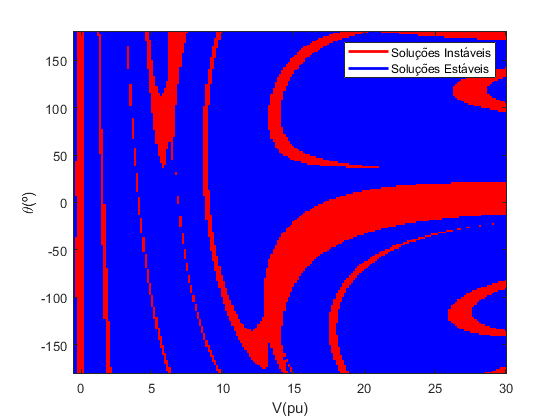
\includegraphics[width=\textwidth]{textuais/capitulo4/figuras/33_FPOM_NOM.png}
        \caption{$\lambda=1$}
    \end{subfigure}
    \vfill
    \begin{subfigure}[b]{0.45\textwidth}
        \centering
        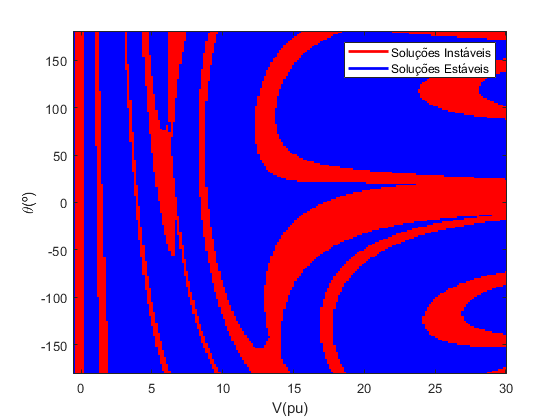
\includegraphics[width=\textwidth]{textuais/capitulo4/figuras/33_FPOM_2lambda.png}
        \caption{$\lambda=2$}
    \end{subfigure}
    \vfill
    \begin{subfigure}[b]{0.45\textwidth}
        \centering
        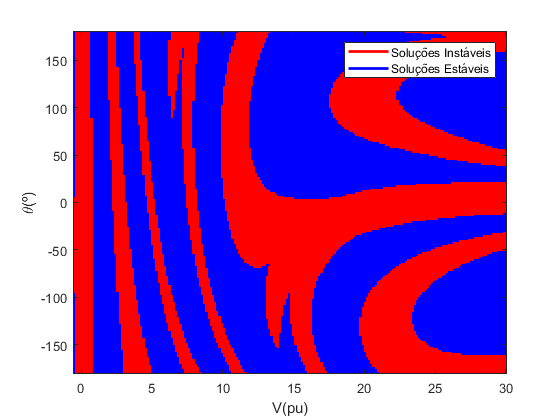
\includegraphics[width=\textwidth]{textuais/capitulo4/figuras/33_FPOM_3lambda.png}
        \caption{$\lambda=3$}
    \end{subfigure}
        \\
   \caption*{Fonte: Elaborada pelo autor}
   \label{fig:FPMO-33}
\end{figure}

\begin{table}[H]
    \centering
    \caption{Área Estável do Mapa Fractal FPMO - IEEE 33 Barras}
    \begin{tabular}{c c c c}
        \toprule
        FPMO & $\lambda = 1$ & $\lambda = 2$ & $\lambda = 3$ \\
        \midrule
        Proporção & $80.99\%$ & $71.89\%$ & $58.24\%$ \\
        \bottomrule
    \end{tabular}
    \caption*{Fonte: Elaborada pelo autor}
    \label{tabela_fractal_FPMO_33}
\end{table}

\clearpage
\begin{figure}[H]
    \centering
    \caption{Mapa Fractal FPPOL - IEEE 33 Barras}
    \begin{subfigure}[b]{0.45\textwidth}
        \centering
        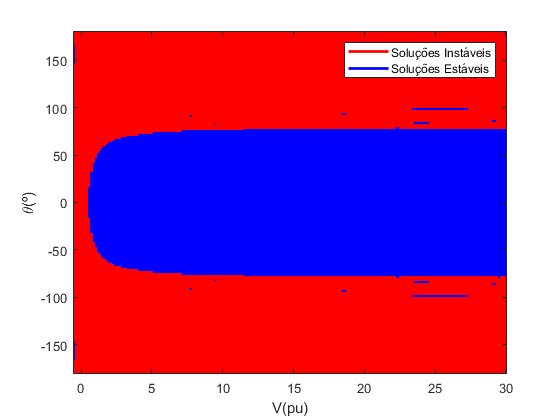
\includegraphics[width=\textwidth]{textuais/capitulo4/figuras/33_FP_POL_NOM.png}
        \caption{$\lambda=1$}
    \end{subfigure}
    \vfill
    \begin{subfigure}[b]{0.45\textwidth}
        \centering
        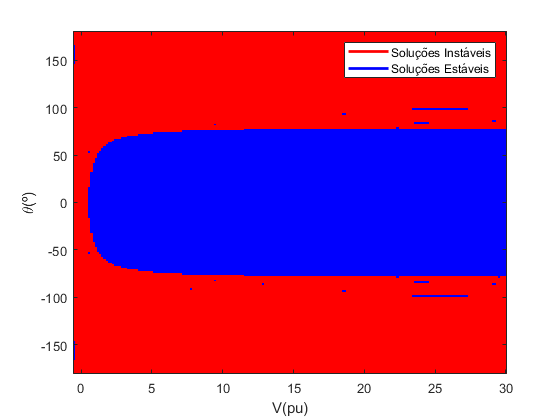
\includegraphics[width=\textwidth]{textuais/capitulo4/figuras/33_FP_POL_2lambda.png}
        \caption{$\lambda=2$}
    \end{subfigure}
    \vfill
    \begin{subfigure}[b]{0.45\textwidth}
        \centering
        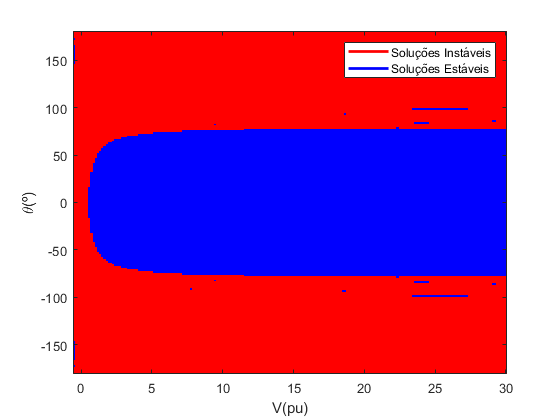
\includegraphics[width=\textwidth]{textuais/capitulo4/figuras/33_FP_POL_3lambda.png}
        \caption{$\lambda=3$}
    \end{subfigure}
        \\
   \caption*{Fonte: Elaborada pelo autor}
   \label{fig:FPPOL-14}
\end{figure}

\begin{table}[H]
    \centering
    \caption{Área Estável do Mapa Fractal FPPOL - IEEE 33 Barras}
    \begin{tabular}{c c c c}
        \toprule
        FPPOL & $\lambda = 1$ & $\lambda = 2$ & $\lambda = 3$ \\
        \midrule
        Proporção & $40.23\%$ & $40.23\%$ & $40.22\%$\\
        \bottomrule
    \end{tabular}
    \caption*{Fonte: Elaborada pelo autor}
    \label{tabela_fractal_FPPOL_33}
\end{table}

\clearpage
\begin{figure}[H]
    \centering
    \caption{Mapa Fractal FPRET - IEEE 33 Barras}
    \begin{subfigure}[b]{0.45\textwidth}
        \centering
        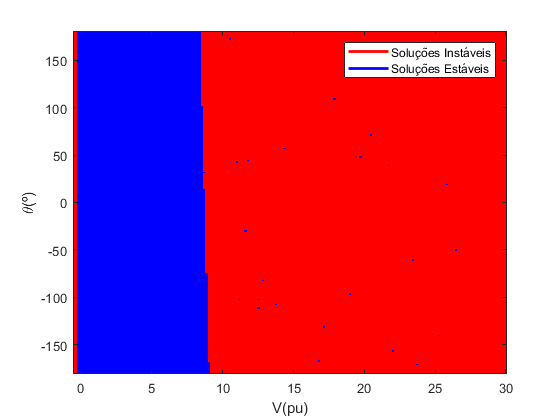
\includegraphics[width=\textwidth]{textuais/capitulo4/figuras/33_FP_RET_NOM.png}
        \caption{$\lambda=1$}
    \end{subfigure}
    \vfill
    \begin{subfigure}[b]{0.45\textwidth}
        \centering
        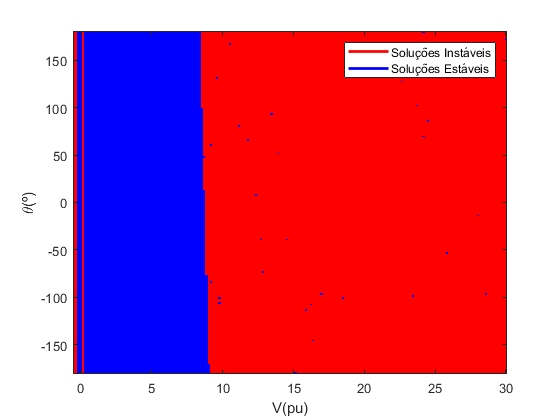
\includegraphics[width=\textwidth]{textuais/capitulo4/figuras/33_FP_RET_2lambda.png}
        \caption{$\lambda=2$}
    \end{subfigure}
    \vfill
    \begin{subfigure}[b]{0.45\textwidth}
        \centering
        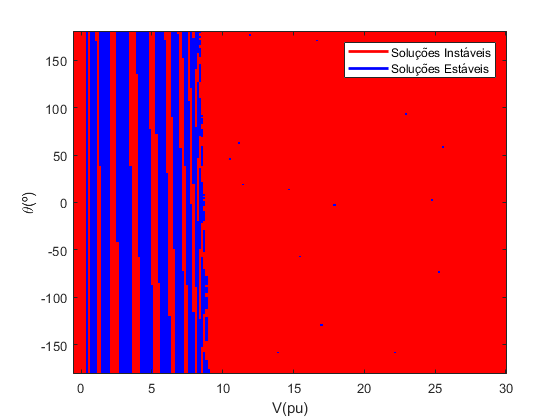
\includegraphics[width=\textwidth]{textuais/capitulo4/figuras/33_FP_RET_3lambda.png}
        \caption{$\lambda=3$}
    \end{subfigure}
        \\
   \caption*{Fonte: Elaborada pelo autor}
   \label{fig:FPRET-33}
\end{figure}

\begin{table}[H]
    \centering
    \caption{Área Estável do Mapa Fractal FPRET - IEEE 33 Barras}
    \begin{tabular}{c c c c}
        \toprule
        FPRET & $\lambda = 1$ & $\lambda = 2$ & $\lambda = 3$ \\
        \midrule
        Proporção & $29.39\%$ & $28.90\%$ & $17.61\%$ \\
        \bottomrule
    \end{tabular}
    \caption*{Fonte: Elaborada pelo autor}
    \label{tabela_fractal_FPRET_33}
\end{table}

\subsection{Tempo Computacional e Número de Iterações}

Foram medidos mil execuções em carga nominal e a média dos tempos computacionais e número de iterações estão registradas na tabela \ref{tabela_tempo_33}.

Constatou-se uma vantagem significante para o método \acs{FPRET} em relação aos outros. Por mais que o \acs{FPMO} tenha tido menor número de iterações, consequência da otimização do próximo passo, seu tempo médio por iteração foi consideravelmente maior, apresentando a pior performance dentre os três métodos.

\begin{table}[H]
    \centering
    \caption{Esforço computacional e iterações - IEEE 33 Barras.}
    \begin{tabular}{c c c }
        \toprule
        Método & Tempo Médio (s)& Número de Iterações Médio \\
        \midrule
        FPMO & 0.0513 & 5 \\
        FPPOL & 0.0389 & 5 \\
        FPRET & 0.0207 & 7 \\
        \bottomrule
    \end{tabular}
    \caption*{Fonte: Elaborada pelo autor}
    \label{tabela_tempo_33}
\end{table}

\subsection{Carregamento Máximo}
Os valores do fator de escala máximo $\lambda$ são apresentados na Tabela \ref{tabela_fatores_escala_33}. Neste caso, foi percebido uma fator de escala maior para o \acs{FPPOL}, seguido do \ac{FPMO} e \ac{FPRET}. 
\begin{table}[H]
\centering
\caption{Fatores de Escala Máximo - IEEE 33 Barras}
\begin{tabular}{c c}
\hline
\textbf{Algoritmo} & \textbf{Fator $\lambda_{max}$} \\
\hline
FPMO &  3.51420 \\
FPPOL & 3.51548 \\
FPRET & 3.51415\\
\hline
\end{tabular}
\label{tabela_fatores_escala_33}
\caption*{Fonte: Elaborada pelo autor}
\end{table}

































\clearpage
\section{RESULTADOS PARA O SISTEMA 14 BARRAS}
O sistema IEEE de 14 barras é um modelo padrão usado para estudos de sistemas de potência, contendo 14 barras, 20 linhas de transmissão, 2 geradores (barras $V\theta$ e $PV$), 3 compensadores síncronos (barras $PV$) e 11 cargas (barras $PQ$). Este sistema representa o sistema elétrico de potência americano da década de 1960. Os dados de barras e de linhas podem ser consultados no apêndice contendo todas as simulações e testes feitos.
\begin{figure}[H]
    \centering
    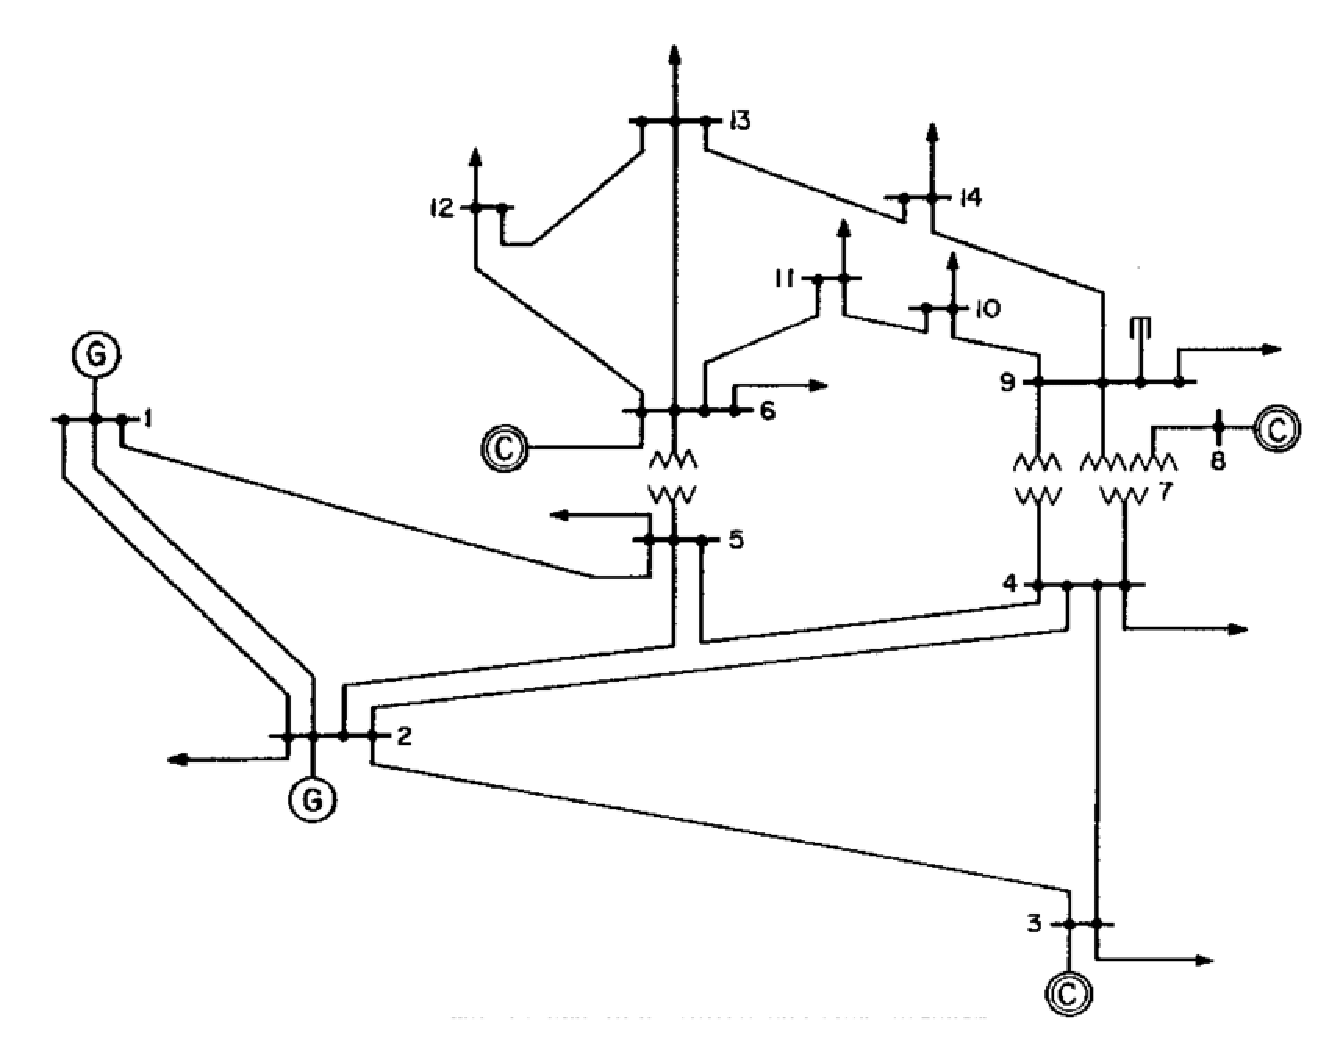
\includegraphics[scale=0.5]{textuais/capitulo4/figuras/IEEE_14BUS.pdf}
    \caption{Topologia do Sistema IEEE 14 Barras}
    \label{fig:enter-label}
\end{figure}

\subsection{Análise Fractal}
Neste sistema também observou-se $100\%$ de região de convergência para a solução do problema ao redor de $1 \angle 0^ \circ$ como palpites iniciais. Da mesma forma que o estudo anterior, optou-se pelo intervalo de $[-0.5, 30]V$ e $[-180, 180]^\circ$ para melhor visualização e comparação dos resultados, além do mesmo número de fluxos rodados por imagem.

\begin{itemize}
    \item As regiões estáveis aumentaram de área com o aumento de carga;
    \item O Mapa Fractal \acs{FPMO} produziu uma área de convergência muito superior aos outros métodos;
    \item Melhor convergência do \acs{FPRET} e \acs{FPMO} em relação aos ângulos de fase como palpites iniciais, maior fraqueza do \acs{FPPOL};
    \item Menor sensibilidade do mapa fractal \acs{FPPOL} com a variação de $\lambda$.
\end{itemize}


\clearpage
\begin{figure}[H]
    \centering
    \caption{Mapa Fractal FPMO - IEEE 14 Barras}
    \begin{subfigure}[b]{0.45\textwidth}
        \centering
        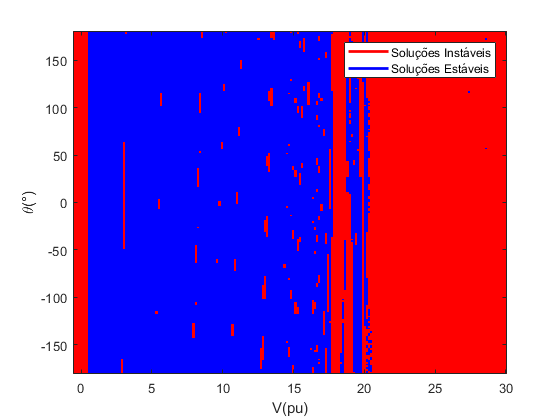
\includegraphics[width=\textwidth]{textuais/capitulo4/figuras/FPOM_nom.png}
        \caption{$\lambda=1$}
    \end{subfigure}
    \vfill
    \begin{subfigure}[b]{0.45\textwidth}
        \centering
        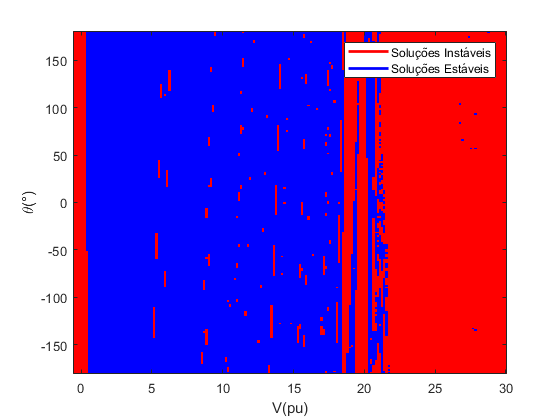
\includegraphics[width=\textwidth]{textuais/capitulo4/figuras/FPOM_10LAMBDA.png}
        \caption{$\lambda=10$}
    \end{subfigure}
    \vfill
    \begin{subfigure}[b]{0.45\textwidth}
        \centering
        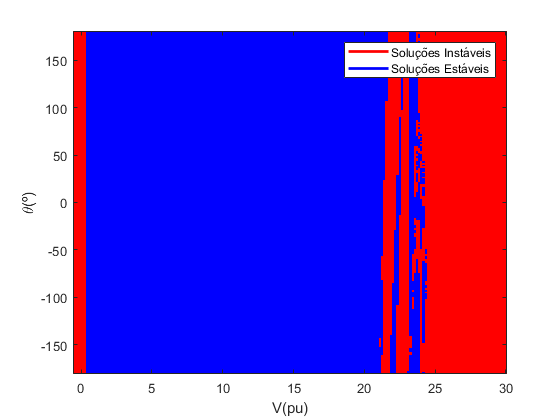
\includegraphics[width=\textwidth]{textuais/capitulo4/figuras/fp_om_20lambda.png}
        \caption{$\lambda=35$}
    \end{subfigure}
        \\
   \caption*{Fonte: Elaborada pelo autor}
   \label{fig:FPMO-14}
\end{figure}

\begin{table}[H]
    \centering
    \caption{Área Estável do Mapa Fractal FPMO - IEEE 14 Barras}
    \begin{tabular}{c c c c}
        \toprule
        FPMO & $\lambda = 1$ & $\lambda = 10$ & $\lambda = 35$ \\
        \midrule
        Proporção & $58.08\%$ & $61.33\%$ & $71.85\%$ \\
        \bottomrule
    \end{tabular}
    \caption*{Fonte: Elaborada pelo autor}
    \label{tabela_fractal_FPMO_14}
\end{table}

\clearpage
\begin{figure}[H]
    \centering
    \caption{Mapa Fractal FPPOL - IEEE 14 Barras}
    \begin{subfigure}[b]{0.45\textwidth}
        \centering
        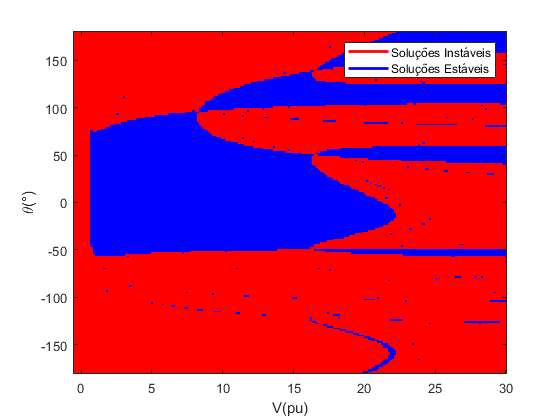
\includegraphics[width=\textwidth]{textuais/capitulo4/figuras/fp_pol_nom.png}
        \caption{$\lambda=1$}
    \end{subfigure}
    \vfill
    \begin{subfigure}[b]{0.45\textwidth}
        \centering
        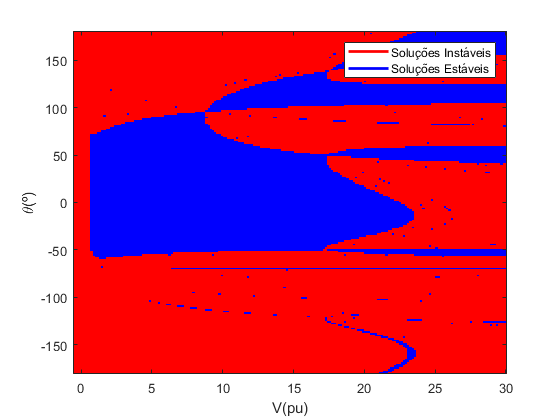
\includegraphics[width=\textwidth]{textuais/capitulo4/figuras/FP_POL_10lambda.png}
        \caption{$\lambda=10$}
    \end{subfigure}
    \vfill
    \begin{subfigure}[b]{0.45\textwidth}
        \centering
        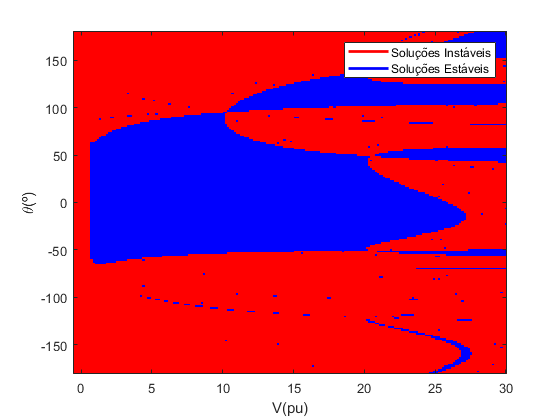
\includegraphics[width=\textwidth]{textuais/capitulo4/figuras/fp_pol_20lambda.png}
        \caption{$\lambda=35$}
    \end{subfigure}
        \\
   \caption*{Fonte: Elaborada pelo autor}
   \label{fig:FPPOL-14}
\end{figure}

\begin{table}[H]
    \centering
    \caption{Área Estável do Mapa Fractal FPPOL - IEEE 14 Barras}
    \begin{tabular}{c c c c}
        \toprule
        FPPOL & $\lambda = 1$ & $\lambda = 10$ & $\lambda = 35$ \\
        \midrule
        Proporção & $30.81\%$ & $31.98\%$ & $33.57\%$\\
        \bottomrule
    \end{tabular}
    \caption*{Fonte: Elaborada pelo autor}
    \label{tabela_fractal_FPPOL_14}
\end{table}

\clearpage
\begin{figure}[H]
    \centering
    \caption{Mapa Fractal FPRET - IEEE 14 Barras}
    \begin{subfigure}[b]{0.45\textwidth}
        \centering
        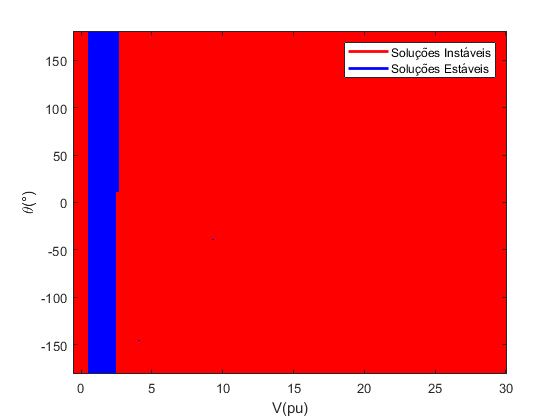
\includegraphics[width=\textwidth]{textuais/capitulo4/figuras/FP_RET_NOM.png}
        \caption{$\lambda=1$}
    \end{subfigure}
    \vfill
    \begin{subfigure}[b]{0.45\textwidth}
        \centering
        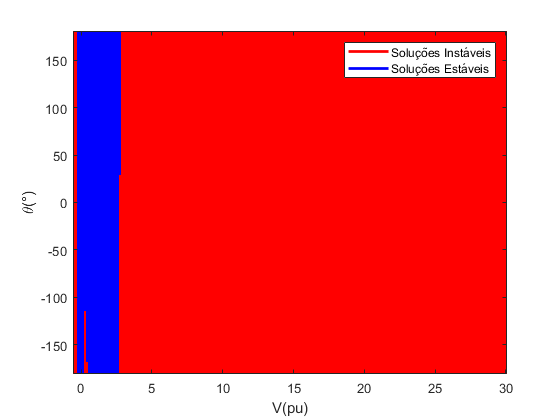
\includegraphics[width=\textwidth]{textuais/capitulo4/figuras/FP_RET_10lambda.png}
        \caption{$\lambda=10$}
    \end{subfigure}
    \vfill
    \begin{subfigure}[b]{0.45\textwidth}
        \centering
        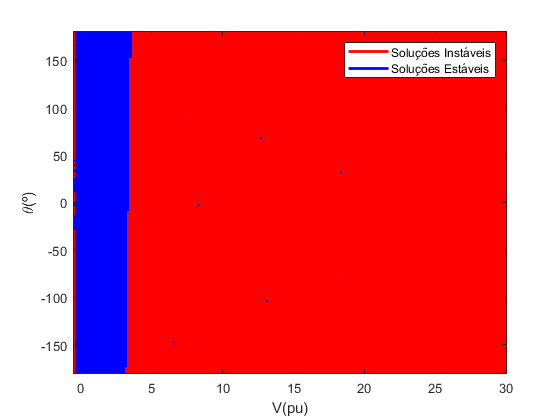
\includegraphics[width=\textwidth]{textuais/capitulo4/figuras/fp_ret_20lambda.png}
        \caption{$\lambda=35$}
    \end{subfigure}
        \\
   \caption*{Fonte: Elaborada pelo autor}
   \label{fig:FPRET-14}
\end{figure}

\begin{table}[H]
    \centering
    \caption{Área Estável do Mapa Fractal FPRET - IEEE 14 Barras}
    \begin{tabular}{c c c c}
        \toprule
        FPRET & $\lambda = 1$ & $\lambda = 10$ & $\lambda = 35$ \\
        \midrule
        Proporção & $6.74\%$ & $9.60\%$ & $12.37\%$ \\
        \bottomrule
    \end{tabular}
    \caption*{Fonte: Elaborada pelo autor}
    \label{tabela_fractal_FPRET_14}
\end{table}


\subsection{Tempo Computacional e Número de Iterações}

Foi observado uma vantagem do \ac{FPRET} em relação a todos os métodos. Nota-se que o \ac{FPMO} reduz o número de iterações médio, mas o tempo adicional de seus cálculos trouxe uma performance geral menor, assim como foi evidenciado para o sistema IEEE 33 Barras.


Na tabela \ref{tabela_tempo_14}, resultado de mil execuções com carregamento nominal, encontram-se os valores de tempo médio e de iterações de cada método para o IEEE 14 Barras. 

\begin{table}[H]
    \centering
    \caption{Esforço computacional e iterações - IEEE 14 Barras.}
    \begin{tabular}{c c c }
        \toprule
        Método & Tempo Médio (s)& Número de Iterações Médio \\
        \midrule
        FPMO & 0.0420 & 6 \\
        FPPOL & 0.0284 & 5 \\
        FPRET & 0.0188 & 7 \\
        \bottomrule
    \end{tabular}
    \caption*{Fonte: Elaborada pelo autor}
    \label{tabela_tempo_14}
\end{table}

\subsection{Carregamento Máximo}
Os valores do fator de escala máximo $\lambda$ são apresentados na Tabela \ref{tabela_fatores_escala_14}. Neste caso, os algoritmos FPRET e FPMO mostraram desempenho praticamente idêntico, apresentando uma diferença a partir da nona casa decimal. Isso indica que ambos os métodos têm uma precisão muito próxima quando sujeitos ao mesmo teste de aumento gradual da carga até a divergência. Em contraste, o método em coordenadas polares obteve um fator de escala ligeiramente menor, indicando uma menor performance comparativa neste cenário específico.


\begin{table}[H]
\centering
\caption{Fatores de Escala Máximo - IEEE 14 Barras}
\begin{tabular}{c c}
\hline
\textbf{Algoritmo} & \textbf{Fator $\lambda_{max}$} \\
\hline
FPMO  & 39.603194459 \\
FPPOL & 38.401057300 \\
FPRET & 39.603194453 \\
\hline
\end{tabular}
\label{tabela_fatores_escala_14}
\caption*{Fonte: Elaborada pelo autor}
\end{table}



